\renewcommand\thechapter{\Roman{chapter}}
\chapter{Requirements analysis and specification}
\newpage
\addcontentsline{toc}{section}{Introduction}

\section*{Introduction}
In this chapter, we will present our development methodology. Then we will identify the main actors involved in our platform, and analyse the functional and non-functional requirements. We will then present and describe the use cases most relative to the project's objective. Finally, we will present the sequence diagrams of the platform.

\section{Work methodology}
This section's aim is to explain our methodological approach regarding the development process and the chosen modeling language.
\subsection{Development process}
We chose the Unified Process (UP) to carry out this project, as it allows us to monitor progress in terms of time, cost, quality and client satisfaction. This process is an incremental, iterative process that is based on the system architecture.\\
The unified process is done in four phases: inception, elaboration, construction and transition. Each phase repeats a series of iterations a number of times where each iteration is composed of five activities: capturing needs, analysis, design, implementation, and testing.
\begin{figure}[H]
\centering
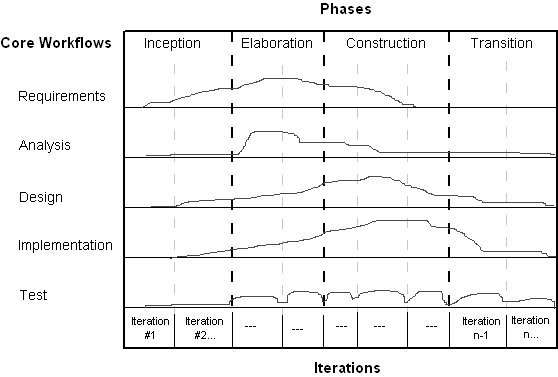
\includegraphics[width=0.7\columnwidth]{Figures/methodo.png}
\caption{Unified process life cycle\cite{methodo}}
\end{figure}
\begin{itemize}
    \item \textbf{Inception}\\
    This is the first phase of the unified process. It is a question of delimiting the scope of the system, meaning, to detect what must appear inside the system and what must remain outside, to identify the actors, to remove any inexactness about the necessary needs and requirements in this phase. It is also a matter building an architecture capable of functioning. In this phase, it is also useful to identify any critical risks that are likely to jeopardize the smooth progress of the project.
    \item \textbf{Elaboration}\\
    After understanding the system, clearing the initial features and functions, specifying the risks, the work to be done now is to stabilize the architecture of the system. This involves refining the initial use case model, even capturing new needs, analyzing and designing most of the use cases formulated, and possibly implementing and testing those initial use cases.
    \item \textbf{Construction}\\
    In this phase we have to try to capture all the remaining needs as it is practically impossible to do in the next phase. Then continue the analysis, design and especially the implementation of all use cases and other diagrams' contents. At the end of this phase, developers must provide an executable and ready version of the system.
    \item \textbf{Transition}\\
    This is the phase that finalizes the product. During this phase, it is necessary to check if the system fully offers the services requested and required by the users, to detect defects, to fill in the gaps in the documentation of the software and to adapt it to the final environment.
\end{itemize}

\subsection{Modeling language}
For a steady and organized application, after choosing the methodology, we need to design our platform using an efficient modeling language. Our choice was Unified modeling language (UML). UML is a language that aids in modeling different artifacts of a system which details the possible scenarios and solutions of our problem.

\section{Actors identification}
Before looking at the platform requirements, we will list the main actors involved. In our case, there are two actors since the platform is used for analysis only.
\begin{itemize}
    \item \textbf{Administrator:}
    This actor has full control over the platform. His role is to manage the users and platform environment. He can add and remove users, update user information or change a user into an admin, manage disk usage, and view logs.
    \item \textbf{Consultant:}
    This actor is an EY employee from the Advanced Cyber Security Team. He gets to analyse E-evidence, using the platform, by providing a file and other information, and can view the results.
\end{itemize}

\section{Requirement specification}
Here we will introduce the platform's different functional and non-functional specifications.
\subsection{Functional specification}
The platform must offer the users the following functions:
\begin{itemize}
    \item \textbf{Authenticate:} Authenticate using credentials.
    \item \textbf{Manage cases:} Add a new case to be analysed, remove existent cases, and consult the list of cases previously added.
    \item \textbf{Check case status:} Check if case is being analysed, done, or unsupported.
    \item \textbf{View case analysis:} Choose a case that is ready and view the analysis reports generated in the platform.
    \item \textbf{Consult administration dashboard:} View admin dashboard that shows general platform information. This function requires the user to be an administrator.
    \item \textbf{Manage Consultants:} Allow an administrator to add, remove or change a consultant's information and role.
    \item \textbf{View session log:} An administrator should be able to View lastly added and removed cases.
    \item \textbf{Logout:} A link to close the current user session.
\end{itemize}
The platform must be secure against the following:
\begin{itemize}
    \item \textbf{Unauthenticated access:} Users must be logged-in to access and use the various platform pages.
    \item \textbf{Unauthorized access:} Users must have access restrictions based on their type, group, or content created.
    \item \textbf{Remote Code Execution:} The application should not be vulnerable to remote code execution through the various commands it uses.
\end{itemize}
\subsection{Non-Functional specification}
Non-functional specifications describe the attributes of the application. In our platform, we have mainly:
\begin{itemize}
    \item \textbf{Availability:} The platform should be accessible when the user needs it.
    \item \textbf{Usability:} The platform must have a user-friendly interface.
    \item \textbf{Performance:} The platform should have quick response time.
    \item \textbf{Portability:} The platform should be easy to move and install on other machines.
\end{itemize}

\section{Platform Design}
This section presents the different UML diagrams modeled to define the platform.
\subsection{Use Case Diagrams presentation}
We will now model the different specifications mentioned earlier using Use Case diagrams. A use case diagram represents a user’s interaction with the system and make it possible to highlight the need of the system user, thus, we will present the most important use cases.\\
But first we will give an overview of the whole application in Figure II.1.
\begin{figure}[H]
\centering
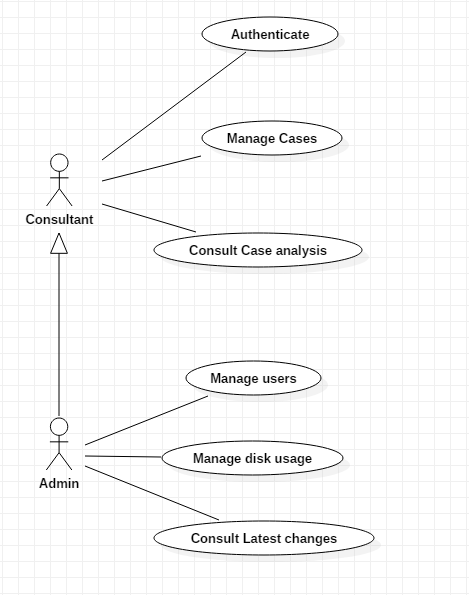
\includegraphics[width=0.6\columnwidth]{Figures/usecase.png}
\caption{Global use case}
\end{figure}
\subsubsection{Case management and analysis}
Figure II.2 shows that an authenticated consultant would be able to use the platform to do the following:
\begin{itemize}
    \item Add a new case: The user will need to provide an evidence file to scan and choose a type of forensics to apply.
    \item Remove a case: The user will be able to select an existent case to be deleted.
    \item Consult case analysis: The user will be able to see reports of extracted data from the provided evidence file regarding the selected case, after the analysis is complete.
\end{itemize}
\begin{figure}[H]
\centering
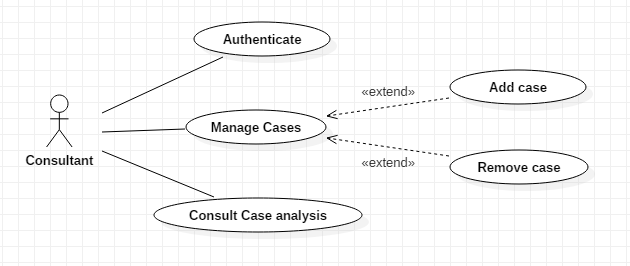
\includegraphics[width=1\columnwidth]{Figures/usecase1.png}
\caption{Case management and analysis use case}
\end{figure}

\subsubsection{Administration}
An Authenticated Administrator, as explained in Figure II.3, would be able to use the platform as an investigator, but also has a unique dashboard that allows him to:
\begin{itemize}
    \item Add a new user: The admin can create a new account for an investigator and fill in his details.
    \item Remove a user: The admin can delete a user account from the platform.
    \item Edit a user: The admin can change a user's account general information or password.
    \item Consult disk usage: The admin, based on the volume used by the application, can choose to clear up space by deleting files from already-analysed cases and temporary files.
    \item Consult log: The admin can see latest changes made in the platform by other users.
\end{itemize}
\begin{figure}[H]
\centering
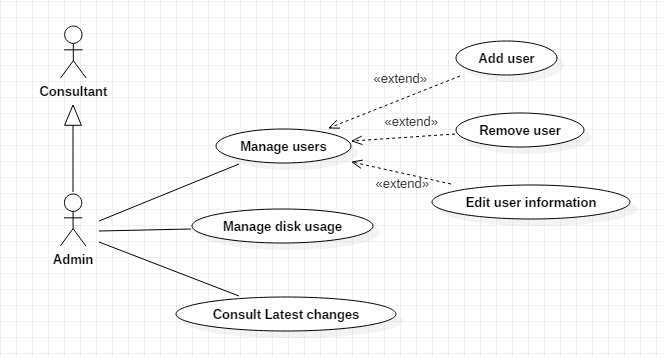
\includegraphics[width=1\columnwidth]{Figures/usecase2.png}
\caption{Administration use case}
\end{figure}

\subsection{Textual description of use cases}
Use case diagrams are useful to give an overview and visualize the interaction between the users and the system, but we also need to give more details about each use case through textual description represented in both Table II.1 and Table II.2. 

\newpage
\begin{longtable}{|p{15cm}|}
\hline
\multicolumn{1}{|c|}{\textbf{Administration use case textual description}}\\
\hline
\multicolumn{1}{|l|}{\textbf{Actor:} } \\
\quad Administrator \\
\multicolumn{1}{|l|}{\textbf{Summary:} } \\
\quad This use case allows the administrator to manage some platform options and the user accounts in it.\\
\multicolumn{1}{|l|}{\textbf{Preconditions:} }\\
\quad Authenticated administrator.\\
\multicolumn{1}{|l|}{\textbf{Scenario:}} \\
\quad - The administrator signs in using his username and password. \\
\quad - The administrator is able to manage cases as a consultant himself. \\
\quad - The administrator views and clears disk usage. \\
\quad - The administrator views the number and the list of users, adds a user, selects a user to change his information or remove him. \\
\quad - The administrator views the latest changes made to the platform by other users. \\
\multicolumn{1}{|l|}{\textbf{Exceptions:}} \\
\quad E1 : incorrect login credentials.\\
\quad 1) The system reloads the login page.\\
\quad E2 : invalid new user information.\\
\quad 2) The system reloads the user modification page.\\
\hline
\caption{\mbox{Description of the "Administration" use case}}
\end{longtable}

\newpage
\begin{longtable}{|p{15cm}|}
\hline
\multicolumn{1}{|c|}{\textbf{Case management and analysis textual description}} \\
\hline
\multicolumn{1}{|l|}{\textbf{Actor:} } \\
\quad Consultant\\
\multicolumn{1}{|l|}{\textbf{Summary:} } \\
\quad This use case allows the consultant to create a new case to analyse an E-evidence, and manage old cases.\\
\multicolumn{1}{|l|}{\textbf{Preconditions:} }\\
\quad Authenticated consultant.\\
\multicolumn{1}{|l|}{\textbf{Scenario:}} \\
\quad - The consultant signs in using his username and password. \\
\quad - The consultant views the list of cases, adds a new case, or removes a case. \\
\quad - The consultant selects a case after the analysis is complete to view extracted data and reports. \\
\multicolumn{1}{|l|}{\textbf{Exceptions:}} \\
\quad E1 : incorrect login credentials.\\
\quad 1) The system reloads the login page.\\
\quad E2 : missing E-evidence file.\\
\quad 2) The system waits for a file to be provided.\\
\quad E3 : Unauthorized access to case.\\
\hline
\caption{\mbox{Description of the "Case management and analysis" use case}}
\end{longtable}

\subsection{Sequence Diagrams}
A sequence diagram, in the UML context, shows the sequence of messages transmitted between the different objects of the application. It is important to highlight the life cycle of each object and the processes that are working simultaneously.\\
We will first present the Authentication's sequence diagram. Then present the system sequence diagram for the analysis phase.\\
The objects used in these sequence diagrams represent a more detailed interaction between the user, the frontend and the backend.\\
The platform follows the MTV pattern followed by Django, which we will understand more later.

\subsubsection{Authentication sequence diagram}
The authentication sequence, on Figure II.4, must occur as first step when accessing the platform to open a user session. This sequence ensures that the user is authenticated to be able to access other areas of the platform.
\begin{figure}[H]
\centering
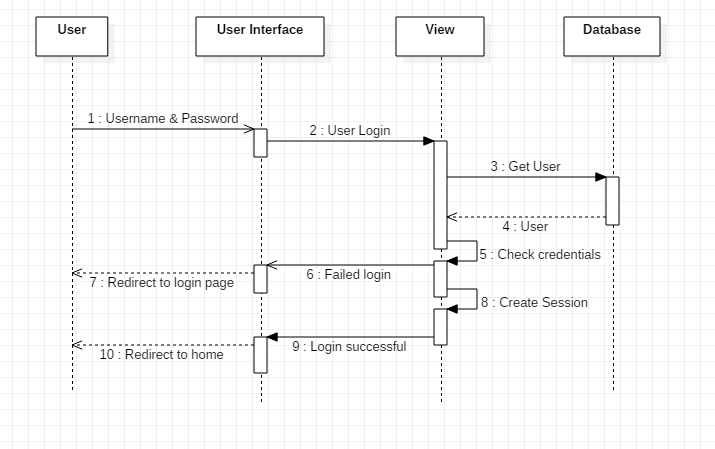
\includegraphics[width=1\columnwidth]{Figures/sequence.png}
\caption{Authentication sequence diagram}
\end{figure}
\textbf{Typical scenario:}\\
- The platform shows a login page.\\
- A user fills in his username and password.\\
- The platform checks the credentials from the database.\\
- The platform creates a session and redirects the user to home page.\\

\subsubsection{Analysis sequence diagram}
An authenticated user will be able to go through the analysis. The analysis sequence diagram that is shown in Figure II.5, is going to be a general overview of how the analysis process from all types of evidence (memory, network, disk).
\begin{figure}[H]
\centering
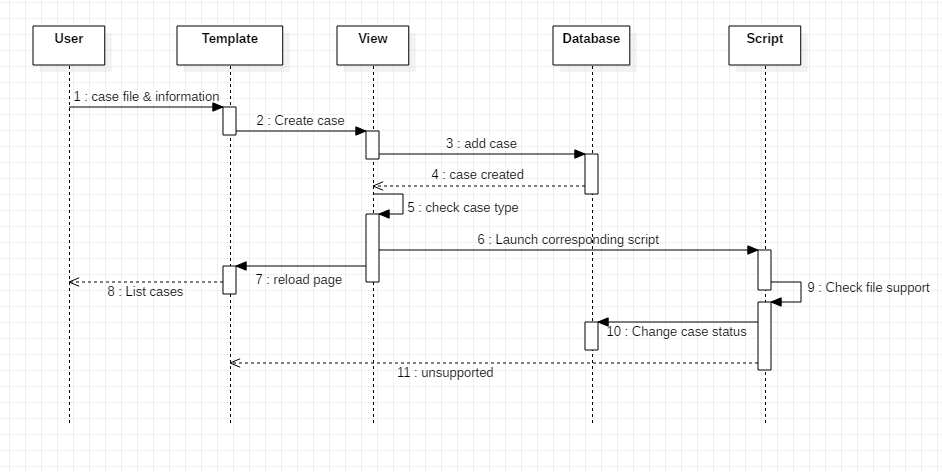
\includegraphics[width=1\columnwidth]{Figures/sequence1.png}
\caption{General analysis sequence diagram}
\end{figure}

Following the previous diagram, the launched script depends on the type of forensic analysis to be run. The system will take care of the analysis using the relative script and output data into the database simultaneously.



\addcontentsline{toc}{section}{Conclusion}
\section*{Conclusion}
Throughout this chapter, we presented and analysed our platform's requirements. We identified the functional and non-functional specifications, then presented the use case and sequence UML diagrams.\\
This chapter paves the way for the next one, in which we will present the implementation of our platform, following the previous analysis.